\title{Simmulation Ideenverbreitung}
%TODO :
\subtitle{IDK ATM}

\author{Arne Struck, Manuel Börries, Jonathan Werner}

\institute{Universität Hamburg \\ 
  Fakultät für Mathematik, Informatik und Naturwissenschaften \\
  Fachbereich Informatik, DKRZ \\
  Praktikum Paralleles Programmieren}
  
\date{\today}

\maketitle

\index{personen}{Struck, Arne}

\begin{abstract}
%TODO content
\quad \\
Aufgabenstellung: \\
Die Erstellung einer parallelen, clusterfähigen Simulation mittels MPI. \\ \\
Projekt Idee: \\
Die Untersuchung der Verbreitung von Meinungen, Vorstellungen innerhalb einer Population.
\keywords{Keywords}
\end{abstract}

\tableofcontents
\newpage
\section{Projekt-Idee}
Diese Projekt soll die Verbreitung und Konkurrenz von Ideen im Sinne einer Weltanschauung, eines kontroversen Themas innerhalb einer begrenzten Population untersuchen und deren Mechanismen simulieren. Die Ideen sollen hierbei durch Kommunikation der Individuen und durch Entwicklung veränderbar sein. \\
Des weiteren darf es keine ''unrealistischen'' Entwicklungen geben. Niemand der gerade erst das Feuer entdeckt hat, baut am nächsten Tag eine Rakete.

\section{Modelierung} %von was?!
In diesem Abschnitt wird ein Überblick über die Modellierung der Ideen, der Welt und der Menschen in ihr gegeben. Details zur eigentlichen Implementation, insbesondere zur Aufteilung auf mehrere Prozesse sind im Abschnitt Implementation zu finden.
\subsection{Die Welt}
\begin{minipage}[t]{0.48\textwidth}
	In 2 Dimensionen betrachtet besteht die Welt auf einem Grid, deren jeweilige Enden miteinander verbunden sind. In einer dreidimensionalen Betrachtung entsteht somit ein Torus-Körper.
\end{minipage}
\begin{minipage}[t]{0.48\textwidth}
	\begin{picture}(0,0)
		\put(20,-75){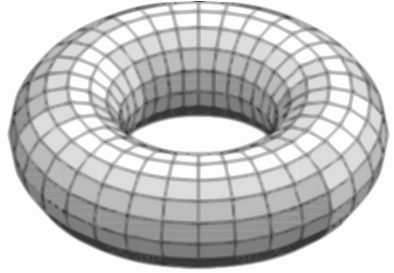
\includegraphics[scale=0.35]{pics/Torus.png}}
	\end{picture}
\end{minipage}	

\subsection{Die Idee}
Eine Idee kann viele Eigenschaften haben, die wichtigen Faktoren um andere Menschen von ihr zu überzeugen lassen sich allerdings grob durch 3 Eigenschaften modellieren. 
Diese sind zum einen die Qualität, die Komplexität, als auch eine arbiträre durch Zahlen ermöglichte Darstellung des Raumes in dem die Idee angesiedelt ist, im folgenden Weltanschauungswert genannt. \\
Die Qualität einer Idee soll den Grad ihrer Überzeugungskraft repräsentieren. 
Die Komplexität hängt mit diesem Wert zusammen, ist allerdings nicht der Selbe, da auch nicht sehr überzeugende Ideen komplex und elaboriert sein können und umgekehrt.

\subsection{Der Mensch}
Ein Mensch besitzt zwei für die Simulation relevante, darstellbare Eigenschaften. 
Die eine ist die Idee, die andere ist ein Weltanschauungswert, ähnlich der der Idee. 
Allerdings repräsentiert der Weltanschauungswert des Menschen s restlichen Ideen, welche er besitzt, die allerdings nicht direkt das Themengebiet der untersuchten Ideen-Gruppe berühren, sondern nur indirekte Einflüsse darauf haben. 
Ein Beispiel hierfür wäre das Mathematikverständnis eines Menschen der Antike betreffend der Frage ob die Erde einer Kugel ähnelt oder nicht.

\subsection{Ablauf}
Zuerst wird eine Population von Menschen mit Ideen durchschnittlich geringer Qualität und Komplexität mit zufälligen Weltanschauungswerten in der Welt geschaffen. 
Die Weltanschauungswerte der Menschen sind in der Nähe ihrer Initialideen angesiedelt. \\
Nun beginnen die verschiedenen Menschen in runden auf der Welt zu ziehen. 
Zu erst wird die Möglichkeit der Entwicklung einer neuen Idee und oder die Veränderung der Weltanschauungswerte evaluiert, diese ist relativ gering, tritt aber dem Gesetz der großen Zahlen folgend bei einigen Individuen alle paar Runden ein. 
Daraufhin werden die Möglichkeiten zur Kommunikation erfasst, sollte ein anderes Individuum sich in Reichweite befinden, wird mit einer gewissen Wahrscheinlichkeit ein Kommunikationsversuch gestartet. 
Die Wahrscheinlichkeit resultiert aus dem menschlichen Verhalten nicht mit jedem Individuum aus seiner Umgebung Konversation zu betreiben.
zum Schluss wird ein Individuum seine Möglichkeiten zur Bewegung evaluieren.

\subsection{Entwicklung}
Die Entwicklung einer Idee erfolgt durch Mutation.
Jeder Mensch hat jede Runde eine Mutationschance sowohl für den Qualitäts-, Komplexitätskomplex, als für den Weltanschauungskomplex.
Beide Mutationen laufen ähnlich ab, zu erst wird eine Richtung gewählt, um zu gewährleisten dass die Eigenschaften nicht in 2 Richtungen mutieren. 
Darauf werden die Mutationsraten der einzelnen Elemente berechnet und diese angepasst.
Bei dem Weltanschauungskomplex existiert noch die finale Absicherung, dass die Differenz beider Werte nicht einen Schwellwert überschreiten.

\subsection{Kommunikation, Konkurrenz und Einschränkungen}
\begin{minipage}[t]{0.48\textwidth}
Bevor es zu einer Kommunikation kommt, muss ein möglicher Kommunikationspartner gefunden werden.
Dieser muss sich (wie rechts dargestellt) in einem benachbartem Feld befinden. 
So können die grüne und die blaue Idee miteinander konkurrieren, der Violetten ist dies allerdings nicht möglich. 
Sollten mehrere Kommunikationspartner zur Verfügung stehen, wird einer diese ausgewählt. \\
Die eigentliche Kommunikation ist in drei Phasen geteilt. 
Nun da ein Kommunikationspartner gefunden ist, wird entschieden ob die beiden sich austauschen.
\end{minipage}
\begin{minipage}[t]{0.48\textwidth}
\begin{picture}(0,0)
		\put(15,-165){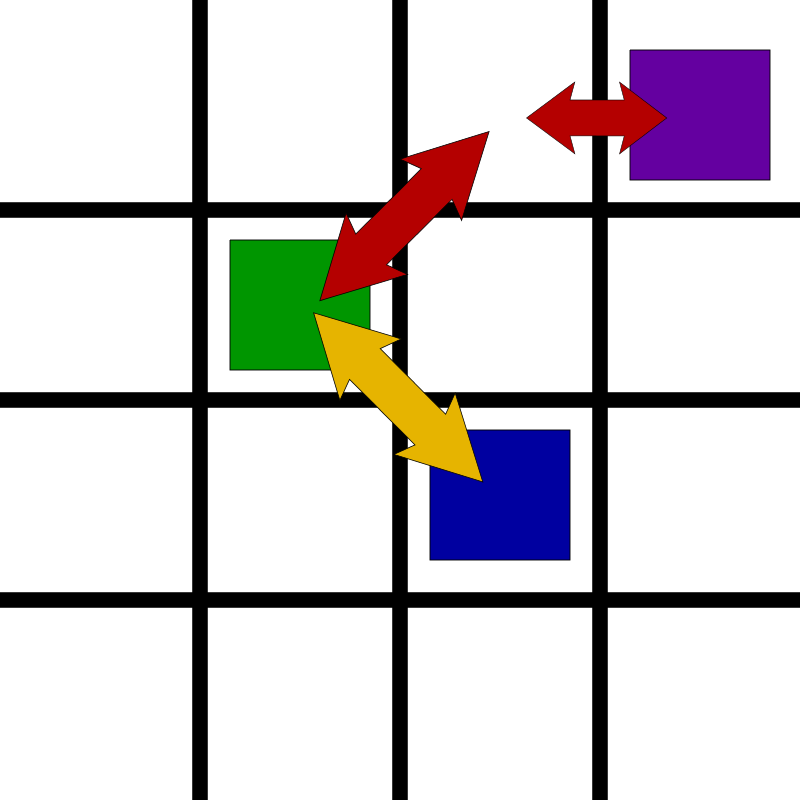
\includegraphics[scale=0.2]{pics/GridComm.png}}
		\put(25,-185){
		\begin{minipage}{0.7\textwidth}
			Kommunikationsmöglichkeiten
		\end{minipage}
		}
\end{picture}
\end{minipage}
\quad \\ \quad \\
Ist dies geschehen und positiv ausgefallen muss berechnet werden, ob sie einander überzeugen können.
Dies hängt von Faktoren, wie der Komplexitätsdifferenz und den Unterschieden zwischen dem Weltanschauungswert der Zielperson und der Ursprungsidee ab. Je höher die Komplexitätsdifferenz ist, desto größer ist die Wahrscheinlichkeit, dass eine Überzeugung fehlschlägt, da davon auszugehen ist, dass die beiden Menschen auf verschiedenen Ebenen denken und somit nicht einig werden. Die Inkompatibilität sich stark unterscheidender Weltanschauungswerte sollte auf der Hand liegen. \\
Sollte eine Kompatibilität festgestellt werden, so muss ermittelt werden, welche der beiden Ideen die andere dominiert. Dies geschieht anhand eines Qualitätsabgleichs mit einem zufälligen temporären Aufschlag auf die Qualitätswerte beider Ideen. Dieser Aufschlag repräsentiert mögliche sonstige Einflüsse wie beispielsweise die Eloquenz des Gegenübers. \\
Wenn nun ein Gewinner feststeht, muss der Verlierer seine Meinung, respektive seine Idee ändern. Dies ist leicht durch die direkte Übernahme zu garantieren. Allerdings muss auch der Weltanschauungswert des verlierenden Menschens an die Idee angepasst werden, da die Idee einen Einfluss auf diesen hat. \\

\subsection{Bewegung}
Nicht alle Menschen gehen einer missionarischen Tätigkeit (welche Anschauung sie auch immer vertreten) sondern vielen anderen Beschäftigungen nach und verbreiten ihre Ideen eher ungerichtet an andere. \\
Nun gäbe es die Möglichkeit diese Tätigkeiten zu simulieren, dies erscheint allerdings in Anbetracht der Projekt-Idee wenig zielführend, daher ist die Wahl der Bewegungsart auf eine zufällige Wahl aus den maximal 9 erreichbaren Feldern gefallen, welche als eine ausreichende Abstraktion der anderen Tätigkeiten erscheint.
Natürlich existieren auch Missionare in dem Sinn, dass sie ihre Idee einer breiten Masse zugänglich machen, allerdings muss ein zu überzeugender Mensch erst einmal (zum Beispiel durch Mundpropaganda oder zufällige Entdeckung, wenn der Missionar noch unbekannt ist) auf diese Missionare stoßen.
Somit stellt dies kein Argument für die Einschränkung einer zufälligen Bewegung dar. \\ \\
\begin{minipage}[t]{0.38\textwidth}
Die möglichen Bewegungen sind hier noch einmal grafisch in rot zu sehen dargestellt (die Möglichkeit still zu stehen bleibt bestehen, obwohl nicht markiert). \\
\end{minipage}
\begin{minipage}[t]{0.58\textwidth}
\begin{picture}(0,0)
		\put(30,-120){
\includegraphics[scale=0.3]{pics/GridMov.png}}
\end{picture}
\end{minipage}


\section{Implementation}
\subsection{Logik und Idee \& Mensch}
Die im Abschnitt Modellierung geschilderten Modellierungen sind mit einer Ausnahme eins zu eins in Software umgesetzt, wobei die verschiedenen Grenzen und Wahrscheinlichkeiten modifiziert werden können. Die Ausnahme betrifft die Repräsentation eines Menschen und seiner Idee, diese sind durch einen struct mit 4 Feldern repräsentiert, wobei noch ein weiteres Feld als Flag für eine empty-idea hinzukommt.

\subsection{Parallelisierungsschema}

Das Feld wird implementiert durch ein 2D-Array über den struct Ideas.

\begin{verbatim}
#define malloc_idea_matrix(name)                              
    Idea **name = (Idea **)malloc(num_rows * sizeof(Idea *)); 
    for (int i = 0; i < num_rows; ++i)                        
        name[i] = (Idea *)malloc(num_cols * sizeof(Idea)); 
\end{verbatim}
\quad \\
Es werden \textit{zwei} Felder erstellt:

\begin{verbatim}
malloc_idea_matrix(field)
malloc_idea_matrix(field_new)
\end{verbatim}
\quad \\
\texttt{field} wird daraufhin mit leeren Ideen initialisiert und an zufälligen Positionen werden Ideen gespawnt. 
Der Inhalt von \texttt{field} wird dann in \texttt{field\_new} kopiert. 
Man braucht diese zwei Felder, damit eine Idee nur ein mal pro Runde ziehen kann: 
es wird über den Inhalt von \texttt{field} iteriert, der Zug Ideen wird in \texttt{field\_new} vermerkt. 
Somit ist erreicht, dass eine die Idee nach rechts zog, im nächsten Iterationsschritt nicht noch einmal zum Zuge kommen. 
Das Kopieren der Felder ist wie folgt implementiert:

\begin{verbatim}
#define copy_field_into_field_new()        
    for_every(i, num_rows, {               
        for_every(j, num_cols, {           
            field_new[i][j] = field[i][j]; 
          });                              
    });
\end{verbatim}
\quad \\
Der Versuch dies mittels \texttt{memcpy} effizienter zu gestalten schlug fehl, da \texttt{memcpy} bei 2D-Arrays nur die Pointer der Arrays der zweiten Ebene kopiert werden. 
Dies ist allerdings nicht im Interesse des Programmes, da die Ideen by value kopiert werden müssen. \\
\newpage
\quad \\
Die Aufteilung des 2D-Arrays auf die MPI-Prozesse funktioniert per horizontaler Spaltung des Feldes.
Dies bringt die Vorteile einer schnellen Aufteilung und Reduktion der Anzahl an Kanten, welche kommuniziert werden müssen.
Die Ränder bestehen aus \textit{ghost rows}, wobei eine \textit{ghost row} des aktuellen \textit{ranks} der vorletzten Reihe des benachbarten \textit{ranks} entspricht. Die Kommunikation besteht im Austausch der \textit{real} und der \textit{ghost rows} mit den jeweiligen Nachbarn.

\begin{figure}[htbp]
\centering
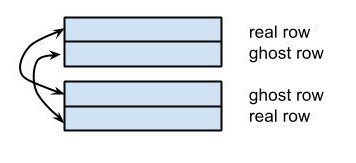
\includegraphics[scale=1]{pics/real-ghost-rows.jpg}
\end{figure}
\quad \\
Dies ermöglicht, jedem Prozess seine Züge unabhängig von den anderen Prozessen durchzuführen. 
Wenn eine Idee auf einer \textit{real row} nach oben respektive nach unten zieht, so hat sie garantiert die Informationen, welche Werte sich in der Zielzelle aus dem Nachbarprozess befinden. \\
Aus diesem Vorgehen resultiert das Konzept der \textit{dependent rows} an den Rändern und der \textit{independent rows} in der Mitte. \\
\textit{Dependend} bedeutet, dass die Ereignisse betreffend Ideen die anliegenden \textit{ranks} betreffen können. 
Die drei äußersten \textit{rows} an den Rändern sind jeweils \textit{dependent}: 
Die beiden äußeren müssen direkt mit dem Nachbarn kommunizieren und die Drittäußerste kann durch Interaktion von Ideen mit der zweitäußersten \textit{row} ebenso \textit{dependet} sein.  \\
Die restlichen \textit{rows} hingegen tangieren die anderen \textit{ranks} nicht innerhalb einer Runde, denn pro Runde kann eine Idee nur ein Feld weiter ziehen. 
Somit können diese \textit{rows} als \textit{independent} gelten.
\newpage

\begin{figure}[t]
\centering
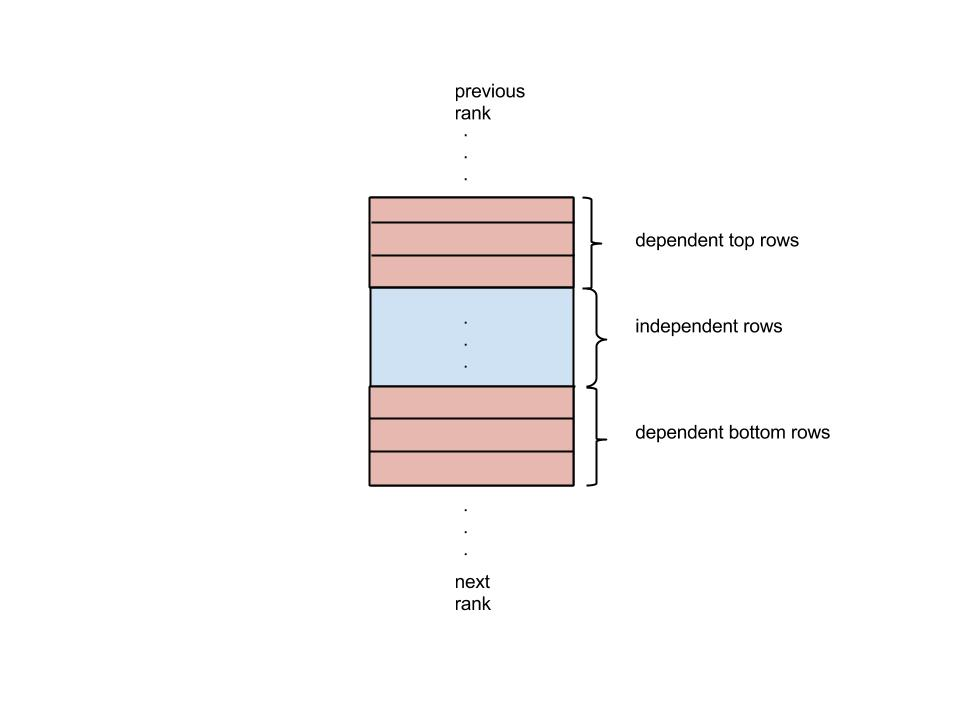
\includegraphics[scale=0.6]{pics/dependent-rows.jpg}
\end{figure}
\quad \\
Daraus folgt, dass die Berechnung der Ereignisse im Feldabschnitt der \textit{independent rows} unabhängig von anderen \textit{ranks} erfolgen kann, die der \textit{dependent rows} allerdings nicht und somit zeitlich orchestriert werden muss.
Diese Orchestration erfolgt in drei Schritten, diese Schritte sehen wie folgt aus und gelten für jeden \textit{rank}.

\begin{enumerate}
	\item Bewege die Ideen die sich auf den \textit{independent rows} befinden.
	\item Bewege die Ideen, die sich auf den \textit{dependent top rows} befinden:
	\begin{enumerate}
  		\item[1.] Sende \textit{top real} und \textit{top ghost row} zu oberem Nachbarn.
  		\item[2.] Empfange \textit{top real} und \textit{top ghost row} von unterem Nachbarn.
	\end{enumerate}
	\item Analog wie Schritt 2 für die \textit{bottom dependent rows}.
\end{enumerate}
\quad \\
Die Kommunikation zwischen den \textit{ranks} wird mittels \texttt{MPI\_Isend} und \texttt{Irecv} realisiert. Dies hat den Vorteil, dass real und \textit{ghost row} nacheinander versendet werden, ohne erst auf die Empfangsbestätigung für das erste Paket zu warten. \\ 
\newpage
\quad \\
Im Code sieht das wie folgt aus: \\
\begin{verbatim}
#define send_ideas(ideas_arr, to, tag, req) \
  MPI_Isend(ideas_arr, num_cols, mpi_idea_type, to, tag, MPI_COMM_WORLD, &req) 

#define receive_ideas_into(ideas_arr, from, tag, req) \
  MPI_Irecv(ideas_arr, num_cols, mpi_idea_type, from, tag, MPI_COMM_WORLD, &req) 

#define send_top_rows(field) \
  /* send our first ghost row into the bottom real row of the previous rank */ \
  send_ideas(field[0], prev_rank, GHOST, req);                                 \
  /* send our first real row into the bottom ghost row of the previous rank */ \
  send_ideas(field[1], prev_rank, REAL, req2);                                 \

#define receive_into_bottom_rows(field) \
  /* receive first ghost row from next rank into our bottom real row */ \
  receive_ideas_into(field[num_rows-2], next_rank, GHOST, req);         \
  /* receive first real row from next rank into our bottom ghost row */ \
  receive_ideas_into(field[num_rows-1], next_rank, REAL, req2);         \
\end{verbatim}
\quad \\
Der \texttt{mpi\_idea\_type} wird hierbei auf folgende Art definiert: \\
\begin{verbatim}
#define mpi_define_idea_type()                                               \
  int          blocklengths[5] = {1,1,1,1,1};                                \
  MPI_Datatype types[5] = {MPI_INT,MPI_INT,MPI_INT, MPI_INT, MPI_INT};       \
  MPI_Datatype mpi_idea_type;                                                \
  MPI_Aint     offsets[5];                                                   \
  offsets[0] = offsetof(Idea, a);                                            \
  offsets[1] = offsetof(Idea, b);                                            \
  offsets[2] = offsetof(Idea, c);                                            \
  offsets[3] = offsetof(Idea, h);                                            \
  offsets[4] = offsetof(Idea, empty);                                        \
    MPI_Type_create_struct(5, blocklengths, offsets, types, &mpi_idea_type); \
    MPI_Type_commit(&mpi_idea_type);                                         \
\end{verbatim}
\quad \\
Die Kommunikation benutzt \texttt{field\_new} zum Austausch der Daten. Am Ende einer Runde wird dieses pro Prozess in \texttt{field} kopiert. \\
Es ist entscheidend, die einzelnen Schritte per \texttt{MPI\_Barrier} voneinander zu trennen, da ansonsten \textit{race conditions} auftreten können.

\subsection{Visualisierung}
Die Visualisierung erfolgt lokal in einer mit Pygame-Implementation. 
Die Daten werden von C, sofern \texttt{\#define DRAW} gilt, pro Prozess pro Runde in \texttt{src/draw/out/\$round-\$proc} exportiert und im Nachhinein von Python eingelesen. 
Dies hat den entscheidenden Nachteil, dass zum einen der Nutzen des Clusters eingeschränkt ist: 
um diesen zu nutzen und gleichzeitig eine Visualisierung zu ermöglichen, müssen die Output-Files auf dem Cluster generiert und dann nach local kopiert werden. 
Dies geschieht per automatisiertem Deploy script, dass den Quellcode auf den cluster rsync, dort das Programm laufen lässt und darauf die Output-Files wieder per rsync zurück kopiert.
Leider ist die Praktikabilität hiervon sehr eingeschränkt, da größere Dateimengen bewegt werden müssen. 
Somit wird der Performance-Gewinn durch den Cluster unterminiert.
Ein weiterer Nachteil ist, dass es sich hierbei um keine Realtime-Visualisierung handelt, sondern nur ein Replay nach der Berechnung abgespielt wird. \\
\quad \\
Das Problem eine Realtime-Visualisierung scheint aber kein triviales zu sein: 
Schließlich müssten die Daten in einem master rank pro Runde gesammelt werden um sie dann grafisch auszugeben. 
Somit wäre hier ein Bottleneck während der Berechnung geschaffen.
Des weiteren war nicht klar, wie und ob so etwas überhaupt auf dem Cluster - per X-Forwarding - funktionieren würde, weshalb wir uns schlussendlich für die lokale Scripting-Variante entschieden haben.
\newpage

\section{Performance}
Wie zu erwarten, ist die Performance mit aktiviertem IO ca. um den Faktor 80 schlechter als ohne: \\
\\
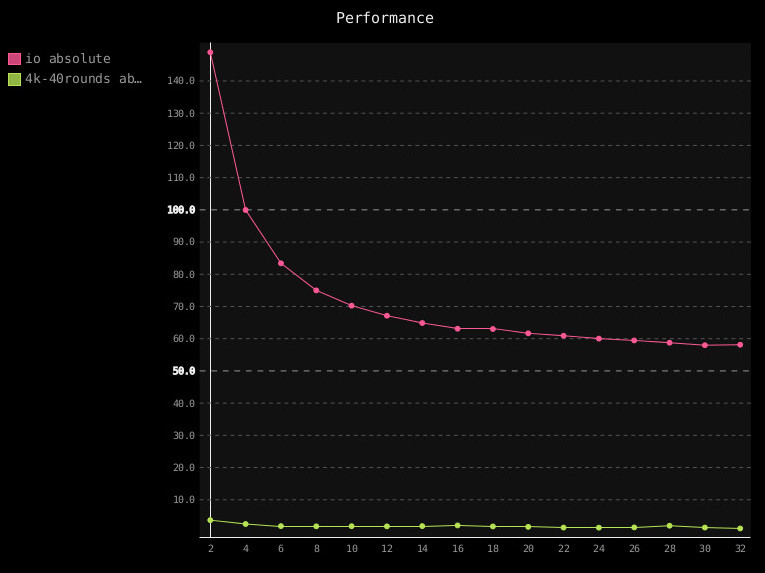
\includegraphics[scale=0.52]{pics/io-vs-no-io-abs.jpg}
\quad \\ \\
Der Speedup der beiden Varianten ähnelt sich aber dennoch. 
Ein Wert von 1 hieße eine lineare Relation zwischen Anzahl von Prozessen und absoluter Geschwindigkeit,
weniger entsprechend weniger effektiv: \\
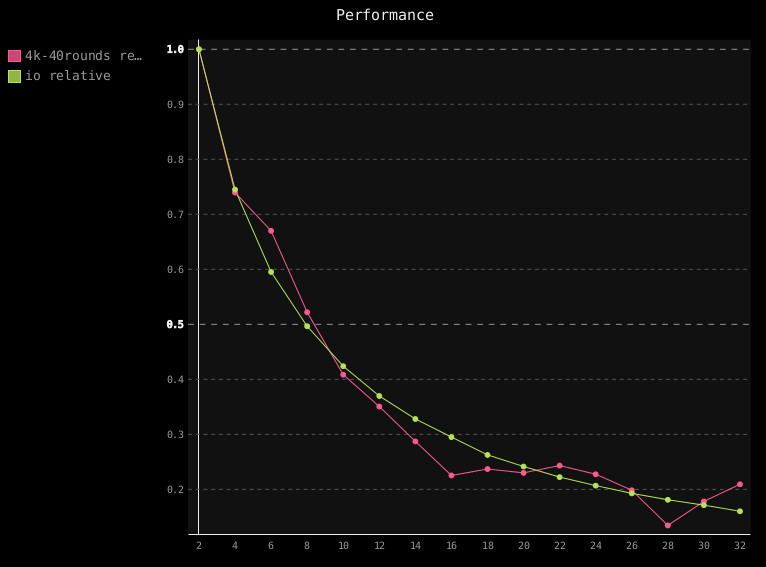
\includegraphics[scale=0.52]{pics/io-vs-no-io-rel.jpg}
\newpage
\quad \\
Der absolute Verlauf ohne IO sieht wie folgt aus: \\ \\
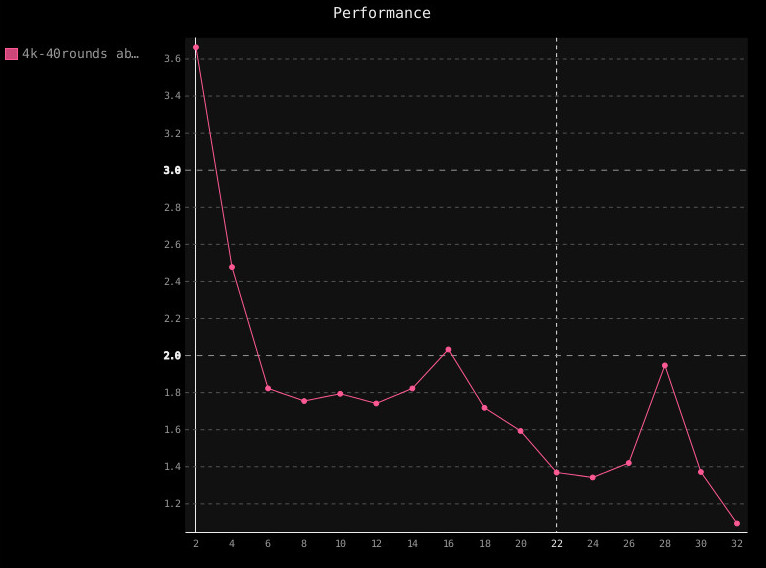
\includegraphics[scale=0.6]{pics/perf-abs.jpg}
\quad \\ \\
Die Ausschläge sind hier relativ stark, sie treten allerdings immer und dann auf, wenn ein zusätzlicher Rechner innerhalb des Clusters hinzugeschaltet wird, da dann ein Overhead an Network-Kommunikation
hinzukommt. \\
Die relativen Speedups und die Abnahme der Effizienz ist damit zu erklären, dass das Verhältnis von MPI-Kommunikation zu realer Rechenzeit steigt und insofern der Anteil an ''teuren'' Instruktionen ständig steigt.

\section{Optimierung und andere Probleme}
Folgende Optimierungen haben wir unter anderem im Laufe der Entwicklung vorgenommen:
\begin{enumerate}
\item \texttt{MPI\_Isend/Recv} anstelle von \texttt{Send/Recv} einsetzen. 
	Dies brachte ca. 10\% Speedup.
\item Den \texttt{field\_new} -\textgreater{} \texttt{field} Kopiervorgang nur einmal ausführen. 
	Dies war Bestandteil eines tieferen Problems, welches uns viele Stunden durch Bugs beschäftigt hat, auch wenn es im Nachhinein trivial wirkt, die ersten Wochen hatten wir das \texttt{field} (und nicht \texttt{field\_new} in der MPI-Kommunikation verschickt. 
	Dies führte zu Korruptionen im Feld, die Ideen vermehrten sich manchmal, bei einer genügend hohen Ideendichte. 
	Durch die Zufälligkeit der Simulation war es quasi unmöglich zu debuggen.
	Erst als wir eine Drop-In Unit-test-artige Bewegungsmethode nutzten, welche Ideen immer nur nach unten gehen ließ, konnten wir den Fehler aufspüren. 
\item Den schon zuvor angesprochenen Versuch, das Kopieren von \texttt{field\_new} in \texttt{field} per \texttt{memcpy} umzusetzen.
	Auch dies funktionierte leider erstmal aus uns unbekannten Gründen, sodass der Eindruck entstand, die Simulation tue das, was sie tuen solle. 
	Leider wurden auf diese Art aber nur Pointer auf die einzelnen rows kopiert. Dies führte zu weiteren schwerwiegenden Bugs.
	\item Genauere und frühzeitige Differenzierung der einzelnen Logik-Fälle und daraus folgende Optimierung der Laufzeit der inneren Schleife.
\end{enumerate}
\quad \\
Generell kann man den Entwicklungsprozess des MPI-Parts anging hauptsächlich als eine Bugsuche, die den Großteil der Zeit extrem in Anspruch war, beschreiben. 
Leider waren Debug-Tools hier nicht wirklich hilfreich, zum einen wegen der Involvierung des Zufalls, die zu nicht reproduzierbaren Ergebnissen führten und somit deterministische Fehlersuche unterminierte, zum anderen, weil erste spezifische Konstellationen des Feldes zu korrupierten Ergebnissen führten. \\
\quad \\
Dementsprechend kann man unsere Strategie bezüglich MPI, als die Funktionsfähigkeit hergestellt war als defensiv beschreiben.
Das System erschien fragil und wir wollten endlich eine funktionierende Basis für das Testen der Simulation mit mehreren Prozessoren an sich haben. 
Daher ist eine Optimierung des MPI-Parts mehr als nicht ausgeschlossen.

%\pagebreak
%\nocite{*}
